\documentclass[11pt]{article}
\usepackage[letterpaper,margin=1in]{geometry}
\usepackage{amsmath,amssymb,amsthm,bm,booktabs,graphicx,microtype}
\usepackage[T1]{fontenc}
\usepackage{lmodern}
\usepackage{xcolor}
\usepackage[colorlinks=true,linkcolor=blue!50!black,citecolor=blue!50!black,urlcolor=blue!50!black]{hyperref}
\usepackage{enumitem}
\setlist{nosep,leftmargin=*}
\newtheorem{theorem}{Theorem}[section]
\newtheorem{proposition}[theorem]{Proposition}
\newtheorem{corollary}[theorem]{Corollary}
\theoremstyle{definition}
\newtheorem{remark}[theorem]{Remark}
\newcommand{\R}{\mathbb{R}}
\newcommand{\norm}[1]{\left\lVert#1\right\rVert}
\newcommand{\ip}[2]{\left\langle#1,#2\right\rangle}
\newcommand{\K}{\mathcal{K}}
\newcommand{\Id}{I}
\newcommand{\F}{\mathcal{F}}
\newcommand{\D}{\mathrm{D}}
\DeclareMathOperator{\diag}{diag}
\DeclareMathOperator{\spanop}{span}
\title{Krylov Transport in Mirror Geometry:\\Finite-Horizon Acceleration of Bregman Iterations}
\author{Joshuah Rainstar}
\date{September 29, 2026\\\small Research draft: foundations and initial experiments}
\begin{document}
\maketitle

\begin{abstract}
A mirror or Bregman iteration transports a state through a geometry determined
by dual coordinates, proximal constraints, and retained memory. We study
advancing this state with a finite polynomial of its local propagator,
compressed by matrix-free Arnoldi iteration. The construction targets a finite
segment of the original evolution and applies to complete deterministic
iteration maps. For smooth mirror descent, we show explicitly that the dual
Jacobian is self-adjoint in the inverse mirror-Hessian metric at every interior
state. For quadratic objectives and quadratic mirrors, the resulting update
is a finite-horizon truncation of a conjugate-gradient Galerkin correction;
an orthogonal error decomposition gives an objective contraction bound.
For nonlinear maps, a discrete trajectory-defect identity separates Krylov
compression from geometric evolution. A boundary-optimum entropy example
shows why finite transport remains meaningful without a finite dual fixed
point. An initial synthetic study measures complete execution cost and
includes stationary Krylov and Anderson comparators. These results formulate
a research program in geometry-aware polynomial transport; they do not
establish a universal acceleration theorem or priority for polynomial
extrapolation, which has substantial prior development.
\end{abstract}

\section{The research object is the iteration state}
Mirror descent, proximal splitting, and split-Bregman methods expose more
structure than a sequence of objective values. An implementation retains a
state whose components determine the next primal estimate, the next dual
driving field, and, in splitting methods, the next memory update. Once this
state is specified, a fixed-parameter deterministic algorithm is a map
\begin{equation}
 z_{j+1}=\F(z_j). \label{eq:map}
\end{equation}
The present question is whether a small number of actions of the local
propagator can replace substantially more applications of $\F$ while retaining
the useful behavior of its trajectory.

The motivating implementation arose in coupled Meyer--Bregman decomposition.
There, the primal variables alone do not close the iteration: the evolving
projected vector fields must also be carried. The finite-flow construction
advanced that complete state with a small projected polynomial. Its broader
mathematical object is not specific to images. Here we develop that object
independently of the decomposition and ask which parts survive across mirror
and splitting geometries.

We distinguish two classes throughout. A smooth mirror-descent map has a
particularly useful dual-coordinate representation and metric. A splitting
map such as ADMM has its own complete state and may be nonsymmetric or
nonnormal. Both admit the finite-flow construction, but the mirror symmetry
result is not automatically a theorem about arbitrary ADMM or split-Bregman
iterations. Likewise, an extrapolated splitting state need not satisfy every
intermediate feasibility property of an ordinary trajectory.

At an anchor $z$, set
\begin{equation}
 r=\F(z)-z,\qquad J=\D\F(z),\qquad
 p_m(t)=\sum_{j=0}^{m-1}t^j. \label{eq:objects}
\end{equation}
The finite-flow proposal is a compressed approximation to $p_m(J)r$.
The polynomial is defined at $t=1$, with $p_m(1)=m$; no stationary inverse is
required. Our central distinction is between three independently assessable
questions: how accurately a frozen local propagator describes the trajectory,
how accurately a small Krylov space represents its polynomial, and whether
the resulting reduction in operator work pays for the extra computation.

\subsection{Prior work and the scope of this draft}
Krylov acceleration of iterative processes is established numerical analysis.
Walker and Ni relate untruncated Anderson acceleration on linear problems to
GMRES \cite{walker}. Regularized nonlinear acceleration constructs improved
solution estimates from past iterates \cite{scieur}. Zhang and White analyze
GMRES acceleration of quadratic ADMM \cite{zhang}. These works preclude a
claim that applying Krylov ideas to Bregman-related iterations is itself new.

Two particularly close precedents determine the present scope. Mai and
Johansson apply Anderson acceleration in the pre-proximal dual coordinates
of Bregman proximal gradient and describe a stabilization rule
\cite{mai}. Poon and Liang analyze local trajectories of splitting methods
and predict future increments with a small fitted recurrence
\cite{poon2019,poon2020}. Their construction includes finite sums of reduced
matrix powers as well as a stationary limit. Thus finite-horizon trajectory
following is also prior art.

This draft investigates a particular combination: \emph{direct current-state
Jacobian actions, Krylov projection in a mirror-derived metric, full-state
transport for coupled iterations, and an explicit separation of nonlinear
and projection errors with complete cost accounting}. The connection to
matrix-function Krylov approximation is classical \cite{saadexp}; the
quadratic analysis below makes its conjugate-gradient content explicit
\cite{saadbook}. Geometric acceleration of Bregman proximal gradient is
also a substantial independent subject \cite{hanzely}. A very recent
preprint studies acceleration through dual geometric updates
\cite{yamashita}; this draft has not completed a theorem-level comparison
with that work. A distinct publication contribution remains to be established
through sharper nonlinear results and matched comparisons with the closest
existing algorithms.

\section{Mirror coordinates expose a symmetric local propagator}
Let $\psi$ be a Legendre mirror on an open convex primal domain, and assume
the required derivatives exist with $\nabla^2\psi(x)\succ0$. For smooth $f$,
an interior mirror-descent step with fixed $\alpha>0$ satisfies
\begin{equation}
 \nabla\psi(x^+)=\nabla\psi(x)-\alpha\nabla f(x).
\end{equation}
With $y=\nabla\psi(x)$ and $x=\nabla\psi^*(y)$, its dual map is
\begin{equation}
 \F(y)=y-\alpha\nabla f(\nabla\psi^*(y)). \label{eq:mirror}
\end{equation}
All coordinates below are genuine local coordinates. On a probability
simplex we use $n-1$ log ratios; the redundant $n$-logit gauge would give a
singular metric.

\begin{proposition}[Local mirror symmetry]\label{prop:symmetry}
At any interior anchor $y$, let
\[
 M=\nabla^2\psi^*(y)=(\nabla^2\psi(x))^{-1},\qquad B=\nabla^2 f(x).
\]
Then
\begin{equation}
 J=I-\alpha BM,\qquad MJ=M-\alpha MBM=(MJ)^T. \label{eq:symmetry}
\end{equation}
Hence $J$ is self-adjoint in $\ip{u}{v}_M=u^TMv$. Its similarity transform is
$M^{1/2}JM^{-1/2}=I-\alpha M^{1/2}BM^{1/2}$.
If $\mu\nabla^2\psi(x)\preceq B\preceq L\nabla^2\psi(x)$,
its spectrum lies in $[1-\alpha L,1-\alpha\mu]$.
\end{proposition}
\begin{proof}
Differentiate \eqref{eq:mirror}. Symmetry follows because both $B$ and $M$
are symmetric. Congruencing the relative Hessian bounds by $M^{1/2}$ gives
the spectral statement. No fixed-point condition was used.
\end{proof}

The statement supplies a principled inner product for Arnoldi. In exact
arithmetic its reduced matrix is symmetric, so a Lanczos implementation is
available. The pilot uses twice-reorthogonalized Arnoldi for numerical
robustness, charging its full cost. Applying $M$ can itself be expensive;
the result is practically useful only when that action is available at an
acceptable cost. The diagonal quadratic and entropy metrics used below
have inexpensive actions.

\subsection{A pre-proximal extension}
For the Bregman proximal-gradient problem $f+g$, with proper closed convex
$g$ and a well-defined unique generalized proximal map, define
\[
 P(y)=\arg\min_x\{\psi(x)+\alpha g(x)-\ip{y}{x}\}.
\]
The complete pre-proximal dual iteration is
\begin{equation}
 \F(y)=\nabla\psi(P(y))-\alpha\nabla f(P(y)). \label{eq:bpg}
\end{equation}
This is the coordinate representation used for dual extrapolation in
\cite{mai}. Wherever $P$ is differentiable with $S=\D P(y)\succ0$,
and $f,\psi$ have symmetric Hessians at $P(y)$,
\begin{equation}
 J=(\nabla^2\psi-\alpha\nabla^2 f)S,
 \qquad SJ=S(\nabla^2\psi-\alpha\nabla^2 f)S=(SJ)^T.
\end{equation}
Thus the same metric construction uses the derivative of the generalized
proximal map. Nonsmooth active constraints can make $S$ rank deficient.
They require an appropriate identified chart or a different positive
metric; the positive-definite statement must not simply be applied to a
singular matrix.

\subsection{What coordinate invariance does and does not mean}
Under an invertible affine coordinate change $\widetilde z=Cz+a$, transform
$\widetilde J=CJC^{-1}$, $\widetilde r=Cr$, and
$\widetilde M=C^{-T}MC^{-1}$. Weighted Arnoldi then produces the same
physical displacement: $\widetilde\delta=C\delta$. This follows by
transforming every inner product and action. Euclidean Arnoldi generally
lacks this invariance under nonorthogonal rescaling. Nonlinear coordinate
changes do not preserve a finite frozen-Jacobian polynomial in this way;
choosing primal or dual coordinates is a substantive modeling decision.

\section{Finite-horizon Arnoldi transport}
Fix an SPD metric $M$ at the anchor and write $\beta=\norm{r}_M$.
If $r=0$, the anchor is unchanged. Otherwise construct an $M$-orthonormal
basis of
\[
 \K_k(J,r)=\spanop\{r,Jr,\ldots,J^{k-1}r\}.
\]
Let $Q^TMQ=I$, $Qe_1=r/\beta$, and $H=Q^TMJQ$. The proposal is
\begin{equation}
 \widehat z_m=z+\delta_{k,m},\qquad
 \delta_{k,m}=\beta Qp_m(H)e_1. \label{eq:proposal}
\end{equation}
Only actions of $J$ are required. The reduced polynomial is evaluated by
$c_0=0$, $c_{j+1}=\beta e_1+Hc_j$, $\delta_{k,m}=Qc_m$.
This recurrence does not invert $I-H$ and remains well-defined for unit
eigenvalues and Jordan blocks. For large horizons, the pair
$(H^m,p_m(H))$ also admits binary composition; the simple pilot uses the
short recurrence with $m=16$.

\begin{proposition}[Affine exactness]\label{prop:affine}
If $\F(w)=Jw+b$ on the complete visited trajectory, then
\begin{equation}
 \F^m(z)-z=p_m(J)r. \label{eq:affine}
\end{equation}
In exact arithmetic, \eqref{eq:proposal} equals this displacement whenever
$m\leq k$. If the Krylov space closes, $JQ=QH$, it equals it for every
nonnegative integer horizon.
\end{proposition}
\begin{proof}
The increments obey $r_{j+1}=Jr_j$, giving \eqref{eq:affine} by summation.
Arnoldi reproduces $J^jr=\beta QH^je_1$ for $j<k$. Invariance of the
closed space extends the equality to all $j$.
\end{proof}

The affine hypothesis concerns the full map on the relevant region.
An unchanged inside/outside mask for a Euclidean disk projection does not
make its exterior branch affine. Nor is a direction-dependent finite secant
a linear Jacobian action; inserting a different secant operator at each
Arnoldi call invalidates the fixed-operator polynomial argument.

\subsection{A reproducible restart rule}
The initial study uses four ordinary steps, then repeatedly constructs a
depth-four, horizon-sixteen proposal and takes one ordinary step from it.
It reacquires the local Jacobian at the next anchor. There is no memory
refresh, objective acceptance gate, adaptive horizon, or fitted relaxation
factor. These choices expose both successes and failures of the mechanism.
They are an experimental schedule, not recommended universal constants.

The nominal cost per full-rank block is one map evaluation to obtain $r$,
four tangent actions, one ordinary settling step, and the complete cost of
metric applications, orthogonalization, and reconstruction. With closure at
rank $\ell<4$, only $\ell$ tangent actions are charged. A variable-step or
stochastic algorithm is not covered merely by reusing this formula: its
schedule or randomness changes the map and needs separate treatment.

\section{A quadratic contraction bound and its CG content}
This section identifies precisely the classical linear-algebraic mechanism.
Let $\psi(x)=\tfrac12x^TGx$, $G\succ0$, and
$f(x)-f(x_*)=\tfrac12(x-x_*)^TB(x-x_*)$, $B\succ0$.
Then $y=Gx$, $M=G^{-1}$, and $J=I-\alpha BM$ are constant.
Assume the eigenvalues of $G^{-1/2}BG^{-1/2}$ lie in $[\mu,L]$ and
$0<\alpha\leq 1/L$. Set
\begin{equation}
 q=1-\alpha\mu,\quad \kappa=L/\mu,\quad
 \theta=\frac{\sqrt\kappa-1}{\sqrt\kappa+1},\quad
 W=M(I-J)=\alpha MBM. \label{eq:quadparams}
\end{equation}
The squared $W$-norm of the dual error equals $2\alpha$ times the objective gap.

\begin{theorem}[Finite-horizon Galerkin contraction]\label{thm:cg}
In exact arithmetic, the natural-metric proposal satisfies
\begin{equation}
 \frac{f(\widehat x_m)-f(x_*)}{f(x)-f(x_*)}
 \leq q^{2m}+(1-q^{2m})\min\{1,4\theta^{2k}\},
 \qquad \widehat x_m=G^{-1}\widehat z_m. \label{eq:cgbound}
\end{equation}
More precisely, define the stationary Galerkin correction
\[
 \delta_\infty=\beta Q(I-H)^{-1}e_1,
 \qquad e_\infty=y+\delta_\infty-y_*.
\]
Then the finite-horizon error has the orthogonal decomposition
\begin{equation}
 \norm{y+\delta_{k,m}-y_*}_W^2
 =\norm{e_\infty}_W^2+
   \norm{\delta_{k,m}-\delta_\infty}_W^2. \label{eq:orthogonal}
\end{equation}
\end{theorem}
\begin{proof}
Write $S=I-J$, $e=y-y_*$. Since $r=-Se$ and
$\K_k(J,r)=\K_k(S,r)$, $\delta_\infty$ is the $M$-Galerkin solution of
$S\delta=r$. Thus $Q^TWe_\infty=0$. Both $\delta_{k,m}$ and
$\delta_\infty$ lie in $\operatorname{ran}Q$, proving
\eqref{eq:orthogonal}. The reduced matrix $H$ is symmetric with spectrum
in $[0,q]$, while $Q^TWQ=I-H$. Consequently
\[
 \delta_\infty-\delta_{k,m}
 =\beta QH^m(I-H)^{-1}e_1,
 \qquad
 \norm{\delta_\infty-\delta_{k,m}}_W
 \leq q^m\norm{\delta_\infty}_W.
\]
Galerkin orthogonality also gives
$\norm{e}_W^2=\norm{e_\infty}_W^2+\norm{\delta_\infty}_W^2$.
Combine these identities with the classical CG polynomial bound
\cite{saadbook},
$\norm{e_\infty}_W\leq 2\theta^k\norm{e}_W$,
and with its trivial bound $\norm{e_\infty}_W\leq\norm{e}_W$.
Converting squared energy to objective gap proves \eqref{eq:cgbound}.
\end{proof}

This theorem does not establish a competitor to CG on a fixed quadratic.
The stationary Galerkin correction has no larger energy error than its
finite-horizon truncation. The finite polynomial becomes interesting when
the geometry changes, a finite trajectory is itself the target, or a
stationary local equation is ill-conditioned or inconsistent. On an affine
quadratic, classical CG is a necessary reference point.

\subsection{When a contraction is a computational acceleration}
Let $c$ be the full block cost divided by the cost of one ordinary step in
a specified implementation. An improved macro-step is not sufficient:
the bound in \eqref{eq:cgbound} must beat $q^{2c}$ to improve the corresponding
worst-case contraction per unit cost. A general nonlinear version is equally
explicit. If $\F$ is a $q$-contraction in a common fixed norm and
\[
 \norm{\widehat z_m-\F^m(z)}\leq\varepsilon\norm{z-z_*},
\]
then
\begin{equation}
 \norm{\widehat z_m-z_*}\leq(q^m+\varepsilon)\norm{z-z_*}.
 \label{eq:costcondition}
\end{equation}
A sufficient cost-adjusted advantage is
$\varepsilon<q^c-q^m$, requiring $m>c$.
This is a conditional criterion. It does not supply an inexpensive bound
on $\varepsilon$, prove global contraction, or allow local metrics at
successive anchors to be compared without additional assumptions.

\section{Nonlinear error separates into two measurable defects}
Let $M$ be fixed during one block, let $Q,H$ be the computed projection, and
write $E=JQ-QH$. For exact Arnoldi $E=h_{k+1,k}q_{k+1}e_k^T$; using the
full residual matrix also accounts for floating-point orthogonalization
error. Define
\[
 c_0=0,\quad c_{j+1}=\beta e_1+Hc_j,\quad
 v_j=Qc_j,\quad \widehat z_j=z+v_j.
\]

\begin{theorem}[Discrete trajectory-defect identity]\label{thm:defect}
If all required evaluations are in the domain of $\F$, define
\[
 N(v)=\F(z+v)-\F(z)-Jv.
\]
Then
\begin{equation}
 d_j:=\F(\widehat z_j)-\widehat z_{j+1}
     =N(v_j)+Ec_j. \label{eq:defect}
\end{equation}
If $\F$ is $\ell$-Lipschitz in the fixed $M$-norm between corresponding
actual and predicted points, then
\begin{equation}
 \norm{\F^m(z)-\widehat z_m}_M
 \leq\sum_{j=0}^{m-1}\ell^{m-1-j}
       \big(\norm{N(v_j)}_M+\norm{Ec_j}_M\big). \label{eq:defectbound}
\end{equation}
If the derivative is $K$-Lipschitz in the induced $M$-norm on each segment
from $z$ to $z+v_j$, then $\norm{N(v_j)}_M\leq\tfrac K2\norm{v_j}_M^2$.
\end{theorem}
\begin{proof}
Use $r=\beta Qe_1$ to subtract the reduced recurrence from
$\F(z+v_j)=z+r+Jv_j+N(v_j)$, giving \eqref{eq:defect}.
For $a_j=\F^j(z)-\widehat z_j$,
$a_{j+1}=\F(\F^j(z))-\F(\widehat z_j)+d_j$ and $a_0=0$.
Apply the Lipschitz bound recursively. The derivative-remainder estimate
follows by integrating along the segment.
\end{proof}

Increasing the Krylov dimension addresses $Ec_j$. It cannot in general
remove $N(v_j)$: a larger exact representation of the wrong frozen geometry
still predicts the wrong trajectory. At a nonsmooth crossing,
\eqref{eq:defect} remains an algebraic identity for a selected linear action,
but the quadratic remainder estimate need not hold. Evaluating every $d_j$
requires the very map calls one hopes to avoid. The implementation therefore
uses these quantities only in a separately costed diagnostic, not as a free
runtime certificate.

\subsection{Relating the metric error to a Bregman distance}
For $x_a=\nabla\psi^*(y_a)$ and $x_b=\nabla\psi^*(y_b)$,
\[
 D_\psi(x_a,x_b)=D_{\psi^*}(y_b,y_a).
\]
If the Hessian along the dual segment is bounded by
$aM\preceq\nabla^2\psi^*\preceq bM$, then
\begin{equation}
 \tfrac a2\norm{y_b-y_a}_M^2
 \leq D_\psi(x_a,x_b)
 \leq\tfrac b2\norm{y_b-y_a}_M^2.
\end{equation}
This translates the fixed-metric transport error into the original mirror
geometry when the metric distortion is controlled. It also identifies a
limitation near domain boundaries where the required constants may degenerate.

\section{Two instructive limits}
\subsection{A boundary optimum with no finite dual fixed point}
Consider minimizing $c^Tx$ on the probability simplex using negative-entropy
mirror descent. In log-ratio coordinates $y_i=\log(x_i/x_n)$,
\begin{equation}
 \F(y)=y+r,\quad r_i=-\alpha(c_i-c_n),\quad J=I.
\end{equation}
For nonconstant $c$, the dual iteration has no finite fixed point.
Nevertheless its rank-one Krylov space closes and
\[
 \delta_{1,m}=mr,\qquad
 x_i^{(m)}=\frac{x_i^{(0)}\exp(-m\alpha c_i)}
                       {\sum_j x_j^{(0)}\exp(-m\alpha c_j)}.
\]
With a unique smallest cost, the primal sequence converges to a simplex
vertex. This is an exactly solvable control, not a new linear-programming
algorithm. It establishes that finite-horizon transport does not logically
require a finite stationary dual solution. A projected stationary inverse
$I-H$ is singular here.

\subsection{A smooth convex case where the cost advantage fails}
Let $f(x)=x^4/4$, use the Euclidean mirror, and take the stable ordinary map
$\F(x)=x-0.3x^3$ from $x=1$. A rank-one frozen polynomial with a long
horizon approaches $1-0.3/(1-0.1)=2/3$. After one settling step it is near
$0.578$. Three ordinary steps, matching one map, one tangent, and one
settling action, reach approximately $0.533$. The latter has the smaller
objective. This elementary counterexample rules out unconditional
cost-adjusted acceleration even for a smooth convex descent trajectory.

\section{Initial experimental program}\label{sec:experiments}
The code is independent of the Meyer implementation. Four principal
geometries are generated with known optima: a quadratic objective with an
anisotropic quadratic mirror; a separable entropy objective whose dual
iteration is affine; a coupled entropy-regularized quadratic on the
simplex; and Lasso solved by ADMM. A primal-coordinate representation of
the same separable entropy iteration is a coordinate ablation. A linear
simplex objective supplies the boundary-drift control.

The entropy simplex uses $n-1$ log ratios and the SPD metric
$M=\diag(x_{1:n-1})-x_{1:n-1}x_{1:n-1}^T$.
Its step size uses the global relative-smoothness bound
$L\leq\tfrac12\lambda_{\max}(A)+\tau$ for the chosen quadratic plus
entropy regularizer. This conservative choice is held fixed across methods.
For Lasso, a planted minimizer and a valid $\ell_1$ subgradient determine
the linear term through the KKT equations. ADMM retains both the split
variable and scaled dual memory; its derivative acts on both.

\subsection{An exact ADMM coordinate ablation}
For the Lasso split let $R=(B+\rho I)^{-1}$, let
$d=\operatorname{shrink}_{\lambda/\rho}(s)$ and $b=s-d$.
The pre-shrink variable $s$ reconstructs both fields exactly, and its map is
\begin{equation}
 \F_s(s)=Rq+\rho R(2d-s)+s-d. \label{eq:shadow}
\end{equation}
Starting with zero state, decoding every ordinary shadow iterate reproduces
the full $(d,b)$ iteration. This is the classical Douglas--Rachford shadow
representation, also relevant to trajectory analysis in \cite{poon2020}; it
does not discard memory. On a fixed shrinkage mask $D$, its Jacobian is
\begin{equation}
 J_s=I-\rho R-D+2\rho RD
    =\tfrac12\{I+(2\rho R-I)(2D-I)\}. \label{eq:shadowjac}
\end{equation}
Since $\norm{2D-I}_2=1$ and $\norm{2\rho R-I}_2<1$ for $B\succ0$,
this local action is nonexpansive in the Euclidean norm. The derivative of
the decode on one fixed mask is the isometric embedding
$L=[D^T,(I-D)^T]^T$, with $L^TL=I$. Across mask changes the decode is
nonlinear, and finite frozen-Jacobian extrapolation need not agree between
the two representations. We therefore include a matched shadow-coordinate
screen to distinguish state-graph artifacts from failure of the frozen
geometry itself.

The comparators are ordinary iteration, Euclidean-metric finite flow,
mirror-metric finite flow, a stationary local Krylov correction, and an
unguarded regularized type-II Anderson implementation of depth four.
The stationary comparator replaces $p_m(H)$ with $(I-H)^{-1}$ and uses the
same acquisition and settling schedule. It is a diagnostic comparison,
not an assumed globally convergent Newton method. The Anderson comparator
is not a reproduction of guarded AA-BPG, and neither it nor these pilots
establish superiority to the published trajectory-following methods.

One unit of operator work is one map call or one analytic Jacobian action.
That count is intentionally accompanied by wall time: a tangent action is
not guaranteed to cost the same as a map, and orthogonalization is not free.
Setup is excluded consistently and recorded separately. Timings include
metric acquisition, basis construction, reduced polynomial evaluation,
reconstruction, ordinary settling, and objective checks spaced by sixteen
work units. The stopping target is a known-optimum objective-gap ratio of
$10^{-6}$, available here because the problems are constructed controls.
It is not claimed as an implementable stopping oracle for arbitrary data.
Final full-state residuals are recorded as separate post-run diagnostics.
Timing orders are randomized between methods after warm-up; repeated
timings on one seed measure implementation variability, not independent
problem samples. Failures and budget censoring remain in the records.

\subsection{Measured outcomes}

All retained comparisons in this section use protocol v2 on the M4 Mini CPU, with one BLAS thread. Each primary family has three seeds and five timing repeats per seed; the penalty and shadow screens use three timing repeats. The primary budgets are 16,384 work units at $n=96$ and 32,768 at $n=512$. The penalty screen uses $n=256$ and 16,384 work units. Here $n$ is the primal dimension: the full ADMM state has size $2n$ and simplex dual states have size $n-1$.

\begin{table}[htbp]\centering\small

\begin{tabular}{lr rrrrr}\toprule

Geometry & $n$ & Ordinary & Finite E & Finite M & Stationary & Anderson\\\midrule

Quadratic mirror & 96 & 13.37 & 14.97 & 15.52 & 5.35 & 6.25\\

Entropy, affine dual & 96 & 6.88 & 11.97 & 12.46 & 3.52 & 12.61\\

Entropy simplex & 96 & 51.64 & 31.97 & 37.08 & -- (2/3) & 3.99\\

ADMM Lasso & 96 & 0.21 & 0.53 & 0.52 & 0.49 & 0.56\\

Entropy, primal & 96 & 14.13 & 12.74 & 13.22 & -- (2/3) & 12.46\\

\midrule

Quadratic mirror & 512 & 95.28 & 45.13 & 45.79 & 16.63 & 14.19\\

Entropy simplex & 512 & 1189.58 & 509.29 & 575.57 & -- (2/3) & 40.65\\

ADMM Lasso & 512 & 1.27 & 1.76 & 1.75 & 1.72 & 3.11\\

Boundary drift & 512 & 9.15 & 9.71 & 11.61 & -- (0/3) & 175.17\\

\bottomrule\end{tabular}

\caption{Milliseconds to the $10^{-6}$ objective-gap target. Each cell is the median across three seeds of each seed\textquotesingle s median runtime. E and M denote Euclidean and mirror metrics. A cell with any failure gives the success count instead of a success-only timing. These are small synthetic experiments, not confidence intervals or a universal performance claim.}

\label{tab:times}\end{table}

At $n=512$, the finite Euclidean-metric schedule gives median elapsed-time speedups of 2.11$\times$ on quadratic mirrors and 2.32$\times$ on the coupled entropy simplex, relative to ordinary iteration. The corresponding mirror-metric speedups are 2.08$\times$ and 2.08$\times$. These gains establish a cross-problem mechanism in this pilot. They do not establish an advantage over the strongest comparator: Anderson is substantially faster on these primary smooth examples, and the stationary Krylov correction is faster when it succeeds. The latter misses the target on entropy seed two at both dimensions.

The finite schedules reduce map-equivalent work by about $2.8\times$ on these smooth problems. At $n=96$, overhead eliminates the elapsed-time advantage on quadratic mirrors and the cheap separable entropy control. The added mirror metric does not improve the work-to-target counts in this primary screen; its coordinate covariance and symmetry are structural properties, not a demonstrated additional speedup here. With the well-performing baseline ADMM penalty $\rho=0.1$, the ordinary method reaches the target too quickly to amortize the fixed Krylov schedule.

\begin{figure}[htbp]\centering

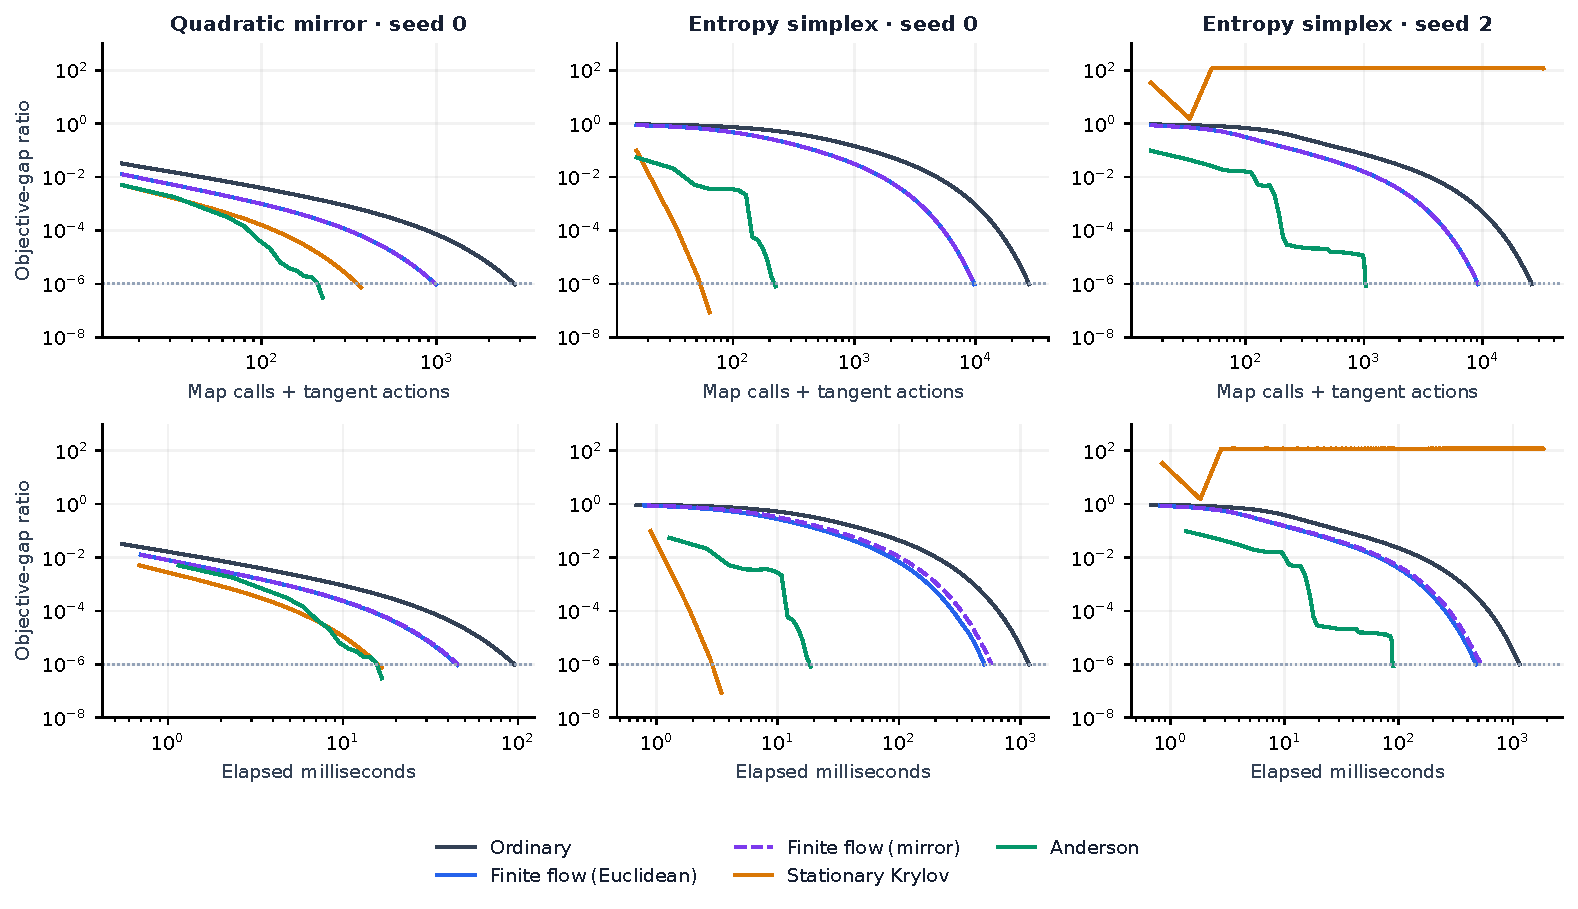
\includegraphics[width=\textwidth]{figures/pilot_curves.pdf}

\caption{Representative primary traces at $n=512$. The top row counts maps and tangent actions; the bottom row uses elapsed time from the first timed repeat. Euclidean and mirror finite-flow work curves nearly coincide. Entropy seed two exposes the stationary comparator\textquotesingle s failure. Tables use all seeds and repeated timing medians.}

\label{fig:curves}\end{figure}

\subsection{Penalty sensitivity and the shadow-coordinate result}

The penalty screen keeps the acceleration schedule fixed. For $\rho=1$, both finite and stationary Krylov schedules fail on all three seeds while ordinary ADMM and Anderson reach the target. At $\rho=10$, finite flow succeeds on only one seed. The exact shadow reparameterization preserves ordinary ADMM numerically and reduces state dimension, but does not resolve these failures. Thus an off-graph extrapolated memory state is not a sufficient explanation: the frozen geometric prediction itself remains inadequate.

\begin{table}[htbp]\centering\small

\begin{tabular}{r rrrrr}\toprule

$\rho$ & Finite, full & Finite, shadow & Stationary, full & Stationary, shadow & AA, shadow\\\midrule

0.001 & 1.52 & 1.70 & 4.19 & 5.63 & 2.44\\

0.01 & 1.28 & 1.41 & 1.65 & 1.45 & 0.92\\

0.1 & 0.55 & 0.61 & 0.57 & 0.62 & 0.64\\

1 & -- (0/3) & -- (0/3) & -- (0/3) & -- (0/3) & 1.23\\

10 & -- (1/3) & -- (1/3) & -- (0/3) & -- (0/3) & 1.85\\

\bottomrule\end{tabular}

\caption{Median elapsed-time speedup relative to ordinary iteration in the same representation, at $n=256$. Values above one are faster. Any unsuccessful seed replaces the ratio by its success count. The full and shadow representations have the same ordinary trajectory and target.}

\label{tab:penalty}\end{table}

\begin{figure}[htbp]\centering

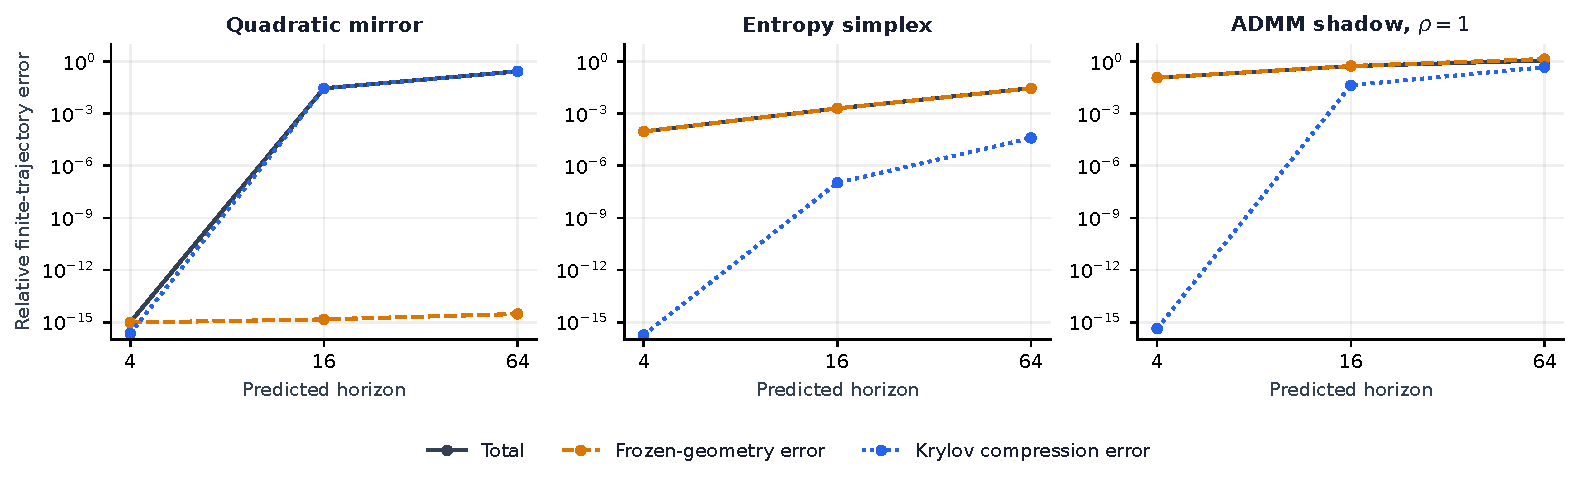
\includegraphics[width=\textwidth]{figures/error_sources.pdf}

\caption{Independent one-block diagnostics at ordinary prefix four, Krylov depth four, seed zero. Errors are normalized by the actual finite displacement; curves at $10^{-16}$ represent the plotting floor. The affine quadratic primarily exposes compression error. Nonlinear and active-mask geometry can dominate in the other examples. All reference map calls and full tangent recurrences used for this figure are separately charged diagnostics, excluded from accelerated solve timings.}

\label{fig:defects}\end{figure}

The boundary-drift control has an exact rank-one finite flow and a singular stationary projected system. Its horizon-sixteen Python implementation still does not beat the extremely cheap ordinary update in elapsed time. This makes the distinction between an exact transport representation and a practical acceleration particularly clear.


\section{What would establish the broader research claim?}
The useful generalization is a statement about a favorable combination of
geometry and cost. A low-dimensional local Krylov space must capture the
relevant finite polynomial; the geometry must remain predictive over the
chosen horizon; the state must contain every variable that drives the next
update; and acquiring and applying the propagator must be cheaper than the
ordinary work it replaces. The preceding propositions make these conditions
explicit, but do not establish that they hold uniformly across Bregman methods.

Three developments would turn the present foundations into a stronger
fundamental result. First, a practical nonlinear bound must control the
trajectory defect without evaluating every skipped step, including active
manifold transitions and degeneration of mirror metrics near boundaries.
Second, a geometric rule for horizon and dimension must be assessed against
fixed choices with its entire acquisition cost charged. Third, independent
problems and faithful implementations of guarded AA-BPG, trajectory-following
extrapolation, and relevant accelerated Bregman baselines must determine
whether direct local actions offer an advantage beyond known methods.

The quadratic identity also suggests an implementation question: when the
mirror metric is cheap and symmetry survives numerically, short-recurrence
Lanczos may reduce the overhead observed in small problems. Conversely,
nonnormal coupled maps require genuine Arnoldi behavior and careful
transient-error analysis. Extending the framework to changing step sizes,
inexact proximal operations, or stochastic gradients requires additional
state and error accounting; none is silently included in the present claim.

The present research contribution is therefore a concrete, testable
formulation of finite transport in mirror geometry, with exact foundations,
explicit classical connections, and a reproducible initial comparison.
The overarching question is which predictable geometric evolutions can be
represented and advanced more cheaply than they can be repeatedly executed.

\appendix
\section{Model definitions and verification}
For the quadratic mirror pilot, $G$ is diagonal with entries spanning
$[1,10^3]$, $B_0=U\diag(\lambda_i)U^T$ with
$\lambda_i\in[10^{-3},1]$, and $B=G^{1/2}B_0G^{1/2}$.
The dual map uses $\alpha=0.9$.
For the positive-orthant entropy control,
\[
 f(x)=\sum_i a_i\{x_i\log(x_i/x_i^*)-x_i+x_i^*\},\quad
 \psi(x)=\sum_i(x_i\log x_i-x_i),
\]
so $y^+=(I-\alpha\diag(a))y+\alpha\diag(a)\log x^*$.
Its primal ablation uses exactly the same ordinary dynamics, expressed
through $x=\exp(y)$.

For the simplex problem,
\[
 f(x)=\tfrac12(x-x^*)^TA(x-x^*)+\tau D_{\mathrm{KL}}(x\Vert x^*),
 \quad A\succ0,\quad \tau=0.05.
\]
The eigenvalues of $A$ span $[n/10^3,n]$, and $x^*$ is a normalized positive
lognormal vector. For Lasso,
\[
 f(x)=\tfrac12x^TBx-q^Tx+\lambda\norm{x}_1,\quad
 q=Bx^*+\lambda s^*,\quad s^*\in\partial\norm{x^*}_1.
\]
The baseline penalty is $\rho=0.1$ and $\lambda=0.05$. The reusable
screened inverse is prepared once for every method. These planted synthetic
families simplify measurement and do not substitute for a natural-data study.

The invariant tests compare analytic Jacobian actions with independent
centered differences, verify mirror symmetry away from stationarity,
check metric coordinate covariance, test Arnoldi polynomial reproduction,
and exercise an invariant Jordan block at eigenvalue one. They verify the
nonlinear defect identity and its Lipschitz bound, the quadratic energy
decomposition and contraction estimate, simplex feasibility, the planted
ADMM KKT point, and the necessity of retained memory. The scalar curvature
counterexample is an explicit negative test. Reproduction commands and
unaltered run records accompany the source.

\begin{thebibliography}{10}
\bibitem{walker} H. F. Walker and P. Ni.
Anderson acceleration for fixed-point iterations.
\emph{SIAM Journal on Numerical Analysis}, 49(4):1715--1735, 2011.
\href{https://doi.org/10.1137/10078356X}{doi:10.1137/10078356X}.

\bibitem{scieur} D. Scieur, A. d'Aspremont, and F. Bach.
Regularized nonlinear acceleration. \emph{NeurIPS}, 2016.
\href{https://arxiv.org/abs/1606.04133}{arXiv:1606.04133}.

\bibitem{zhang} R. Y. Zhang and J. K. White.
GMRES-accelerated ADMM for quadratic objectives.
\emph{SIAM Journal on Optimization}, 28(4):3025--3056, 2018.
\href{https://doi.org/10.1137/16M1059941}{doi:10.1137/16M1059941}.

\bibitem{mai} V. V. Mai and M. Johansson.
Anderson acceleration of proximal gradient methods.
\emph{International Conference on Machine Learning}, 2020.
\href{https://arxiv.org/abs/1910.08590}{arXiv:1910.08590}.

\bibitem{poon2019} C. Poon and J. Liang.
Trajectory of alternating direction method of multipliers and adaptive acceleration.
\emph{NeurIPS}, 2019.
\href{https://arxiv.org/abs/1906.10114}{arXiv:1906.10114}.

\bibitem{poon2020} C. Poon and J. Liang.
Geometry of first-order methods and adaptive acceleration.
Preprint, 2020.
\href{https://arxiv.org/abs/2003.03910}{arXiv:2003.03910}.

\bibitem{saadexp} Y. Saad.
Analysis of some Krylov subspace approximations to the matrix exponential operator.
\emph{SIAM Journal on Numerical Analysis}, 29(1):209--228, 1992.
\href{https://doi.org/10.1137/0729014}{doi:10.1137/0729014}.

\bibitem{saadbook} Y. Saad.
\emph{Iterative Methods for Sparse Linear Systems}, second edition.
SIAM, 2003.
\href{https://www-users.cse.umn.edu/~saad/IterMethBook_2ndEd.pdf}{Author's text}.

\bibitem{hanzely} F. Hanzely, P. Richt\'arik, and L. Xiao.
Accelerated Bregman proximal gradient methods for relatively smooth convex optimization.
\emph{Computational Optimization and Applications}, 2021.
\href{https://doi.org/10.1007/s10589-021-00273-8}{doi:10.1007/s10589-021-00273-8}.

\bibitem{yamashita} Y. Yamashita, S. Takahashi, and A. Takeda.
Accelerated Bregman proximal gradient methods from dual geometric perspectives.
Preprint, September 28, 2026.
\href{https://arxiv.org/abs/2609.34773}{arXiv:2609.34773}.
\end{thebibliography}
\end{document}
